%
% Angepasste FOM Seminarvorlage
%
\documentclass[12pt,a4paper,listof=totoc,bibliography=totoc]{scrartcl}

\usepackage[english]{babel}			% englische Namen/Umlaute
\usepackage[utf8]{inputenc}	    	% Zeichensatzkodierung
\usepackage{silence}
 \WarningFilter{scrartcl}{Usage of package `fancyhdr'}
 \WarningFilter{scrartcl}{Usage of package `parskip'}
\usepackage{fancyhdr}
\usepackage{graphicx}               % Einbinden von Bildern
\usepackage[hidelinks]{hyperref}	% Klickbare Verweise und \autoref{label}
\usepackage[intoc]{nomencl}
\usepackage{setspace}
\usepackage{parskip}
\usepackage{caption}
\usepackage{float}
\usepackage{listings}
\usepackage{scrhack}
\usepackage{geometry}
 \geometry{a4paper, left=40mm, right=20mm, top=40mm, bottom=20mm}
\renewcommand{\familydefault}{\sfdefault}
\renewcommand{\ttdefault}{pcr}
\renewcommand{\lstlistlistingname}{Listings}
\renewcommand{\lstlistingname}{Listing}

% Bildueberschrift oben und rechtsbuendig
\captionsetup{labelfont=bf, textfont=bf}
\captionsetup{justification=raggedright,singlelinecheck=false}

% Blocksatz
\def\justify{%
  \rightskip=0pt
  \spaceskip=0pt
  \xspaceskip=0pt
  \relax
}

%
%	Hier werden Titel, Bearbeiter und das Datum eingetragen
%
\newcommand\svthema{NIS2 \& CIS Controls}
\newcommand\svperson{Christian Frank (\#473088)}
\newcommand\svdatum{\today}
\newcommand\lvname{Cyber Security Management: Sicherheitsstandards \& Reifegradmodelle}
\newcommand\lvtyp{SS 2024}
\newcommand\lvinst{FOM - Hochschule für Oekonomie \& Management}
\newcommand\lvbetr{Friederikos Fotis}

\hypersetup{ % Thema und Author in die Meta-Daten der PDF
  pdftitle={\svthema}, 
  pdfauthor={Christian Frank},
  pdfsubject={Sicherheitsstandards - CIS Benchmarks},
  pdfkeywords={CIS, Benchmarks, NIS2, Security, Kubernetes}
}

\begin{document}

% Titel
\title{ \huge\textbf{\svthema} }
\author{ {\svperson} \\ \svdatum }
\date{ \normalsize \centering 
\includegraphics[width=0.3\textwidth]{FOM}\\ {\lvname} \\ {\lvbetr} \\ {\lvinst} \\ {\lvtyp} }

% Seitennummer oben
\pagestyle{fancy}
\fancyhf{}
\fancyhf[ch]{\thepage}
\renewcommand\headrulewidth{0pt}

\maketitle
\thispagestyle{empty} % laesst die Seitennummer auf der Titelseite verschwinden
\pagenumbering{Roman}

\begin{abstract}
In this paper, we will examine the new NIS2 security standards, compare them to the current set of CIS controls, and evaluate the use of CSI benchmarks to check the readiness of Kubernetes clusters for NIS2 and ensure compliance to mitigate the risks of cyber attacks.

\end{abstract}

\vfill
\begin{figure}[h]
    \centering
    
\includegraphics[]{CC-BY}
\end{figure}

This work is licensed under the Creative Commons Attribution 4.0 International License. To view a copy of this license, visit http://creativecommons.org/licenses/by/4.0/ or send a letter to Creative Commons, PO Box 1866, Mountain View, CA 94042, USA.

\cleardoublepage

\tableofcontents			% Inhaltsverzeichnis
\cleardoublepage

\listoffigures				% Abbildungsverzeichnis
\cleardoublepage

\lstlistoflistings			% Codeverzeichnis
\cleardoublepage

%
% Abkuerzungsverzeichnis
%
\makenomenclature
\renewcommand{\nomname}{List of Abbreviations}

\nomenclature{\textbf{AKS}}{Azure Kubernetes Service}
\nomenclature{\textbf{APA}}{American Psychological Association}
\nomenclature{\textbf{CIS}}{Center for Internet Security}
\nomenclature{\textbf{CISA}}{Cybersecurity and Infrastructure Security Agency}
\nomenclature{\textbf{CNCF}}{Cloud Native Computing Foundation}
\nomenclature{\textbf{CRA}}{Cyber Resilience Act}
\nomenclature{\textbf{ENISA}}{European Union Agency for Cybersecurity}
\nomenclature{\textbf{EU}}{European Union}
\nomenclature{\textbf{EKS}}{Elastic Kubernetes Service}
\nomenclature{\textbf{GKE}}{Google Kubernetes Engine}
\nomenclature{\textbf{IaC}}{Infrastructure as Code}
\nomenclature{\textbf{ICT}}{Information and Communications Technology}
\nomenclature{\textbf{IG}}{Implementation Group}
\nomenclature{\textbf{K8s}}{Kubernetes}
\nomenclature{\textbf{NIS}}{Network and Information Security (Directive)}
\nomenclature{\textbf{NIST}}{National Institute of Standards and Technology}
\nomenclature{\textbf{RKE}}{Rancher Kubernetes Engine}
\nomenclature{\textbf{SOC}}{Security Operations Center}

\printnomenclature[1.5in]          % Abkuerzungsverzeichnis
\cleardoublepage

\pagenumbering{arabic}
\setcounter{page}{5}

%
%	Einfuehrung
%

\pagebreak
\section{Introduction}

\onehalfspacing

\subsection{Cyber Security}

Cybersecurity, also called information security or IT security, is the practice of protecting systems, networks, and programs from digital attacks. It aims to reduce the risk of these attacks and prevent the unauthorized exploitation of systems, networks, and technology.

Cybersecurity is an ongoing process because threats and attack vectors are constantly evolving. Organizations and individuals must proactively implement security measures and stay up-to-date on the latest threats.\footnote{See \textit{Gemini (2024)}: What is Cyber Security. \cite{bardCybersec}}

\subsection{NIS2}

NIS2, which stands for Network and Information Systems Directive II, is the EU's legislative act to strengthen cybersecurity across the European Union. It's essentially an update to the original NIS Directive implemented in 2016.

It sets stricter requirements for various sectors to improve security for essential entities. These entities include organizations in critical sectors like energy, transport, waste management, healthcare, and digital infrastructure providers.

Compared to the original directive, NIS2 applies to a broader range of businesses and organizations; it recognizes the importance of securing the supply chain and includes measures to address vulnerabilities in third-party vendors and suppliers.

It also emphasizes a risk-based approach to cybersecurity. Organizations must identify and assess their security risks and implement appropriate mitigation measures.

NIS2 entered into force on 16 January 2023, and the Member States now have 21 months, until 17 October 2024, to transpose its measures into national law.\footnote{See \textit{Negreiro-Achiaga, M. (2023)}: The NIS2 Directive. \cite{nisBrief}}

\subsection{CIS Controls and Benchmarks}

CIS Controls, or CIS Critical Security Controls, are a prioritized set of best practices designed to improve an organization's cybersecurity posture. Developed by the \href{https://www.cisecurity.org/}{Center for Internet Security} (CIS), a non-profit organization, these controls are a widely trusted framework for defending against cyberattacks.\footnote{See \textit{CIS (2024)}: Critical Security Controls. \cite{cisControls}}

CIS Benchmarks are configuration guides intended to harden various IT systems against cyberattacks based on the CIS' Critical Security Controls. They provide a set of best practices for securing specific operating systems, applications, and cloud platforms. Many of these Benchmarks have specific versions tied to the underlying software version.\footnote{See \textit{CIS (2024)}: Benchmark List. \cite{cisBenchmarks}}

Several platform vendors provide automated tools to check against these benchmarks and report and enforce compliance as a first line of defense.\footnote{See \textit{Rancher (2024)}: CIS Scans. \cite{rancherBenchmarks}}

\subsection{Kubernetes}

Kubernetes, or K8s, is an open-source system designed to automate deploying, scaling, and managing applications built using containers. Containers package software in a standardized unit that includes all dependencies the software needs to run, like code, libraries, and settings. This makes them portable and efficient.

Kubernetes helps manage these containers by grouping them logically. This makes it easier to track and manage complex applications with many containers. The original inspiration for Kubernetes came from Google's internal container orchestration system, Borg.\footnote{See \textit{Gemini (2024)}: What is Kubernetes. \cite{bardKubernetes}} 

In 2015, Kubernetes reached the 1.0 milestone, and in 2016, it was donated to the CNCF; the current release of Kubernetes is 1.30.

"For the people who built it, for the people who release it, and for the furries who keep all of our clusters online, we present to you Kubernetes v1.30: Uwubernetes, the cutest release to date."\footnote{\textit{Dsouza, A. (2024)}: Kubernetes 1.30. \cite{uwubernetes}}

\begin{figure}[H]
\centering
\caption {Kubernetes 1.30 Release Logo}

\includegraphics[width=0.3\linewidth]{images/k8s-1.30.png}
\label{fig:uwubernetes}
\end{figure}

\subsection{Research Question \& Method}

This paper will examine the new NIS2 security standards, compare them to the current CIS controls, and attempt to map them. Once we've established a helpful relationship, we will evaluate using CSI benchmarks to check Kubernetes clusters for compliance. We will also check whether CIS Benchmarks can provide information about the level of compliance for Kubernetes clusters and offer actionable insights into reaching NIS2 compliance.

To do this, we will perform an Experiment and cross-check the findings of several CIS Benchmarks on random clusters against manual evaluation.\footnote{See \textit{Genau, L. (2020)}: Ein Experiment in deiner Abschlussarbeit durchführen. \cite{expScribbr}}

The goal is to establish whether CIS Benchmark results can indicate whether a Kubernetes cluster might be NIS2-compliant as a platform.

\subsection{Gender-neutral Pronouns}

Our society is becoming more open, inclusive, and gender-fluid, and now I think it's time to think about using gender-neutral pronouns in scientific texts, too. Two well-known researchers, Abigail C. Saguy and Juliet A. Williams, both from UCLA, propose to use the singular they/them instead: "The universal singular they is inclusive of people who identify as male, female or nonbinary."\footnote{\textit{Saguy, A. (2020)}: Why We Should All Use They/Them Pronouns. \cite{pronouns}} The aim is to support an inclusive approach in science through gender-neutral language. 

In this paper, I'll attempt to follow this suggestion and invite all my readers to do the same for future articles. Thank you!

If you're not sure about the definitions of gender and sex and how to use them, have a look at the definitions\footnote{See \textit{APA (2021)}: Definitions Related to Sexual Orientation. \cite{apaDefinitions}} by the American Psychological Association.

\subsection{Climate Emergency}

As Professor Rahmstorf puts it: "Without immediate, decisive climate protection measures, my children currently attending high school could already experience a 3-degree warmer Earth. No one can say exactly what this world would look like—it would be too far outside the entire experience of human history. But almost certainly, this earth would be full of horrors for the people who would have to experience it."\footnote{\textit{Rahmstorf, A. (2024)}: Climate and Weather at 3 Degrees More. \cite{3dgreesMore}}


%
%	Begrifflichkeiten
%

\pagebreak
\section{NIS2}

\onehalfspacing

\subsection{The Network and Information Security Directive}

\subsection{Methodology}

\subsection{Center for Internet Security}

\subsubsection{CIS Controls}

\subsubsection{CIS Benchmarks}

\subsection{Rancher}

\begin{figure}[H]
\centering
\caption {Rancher Dashboard}
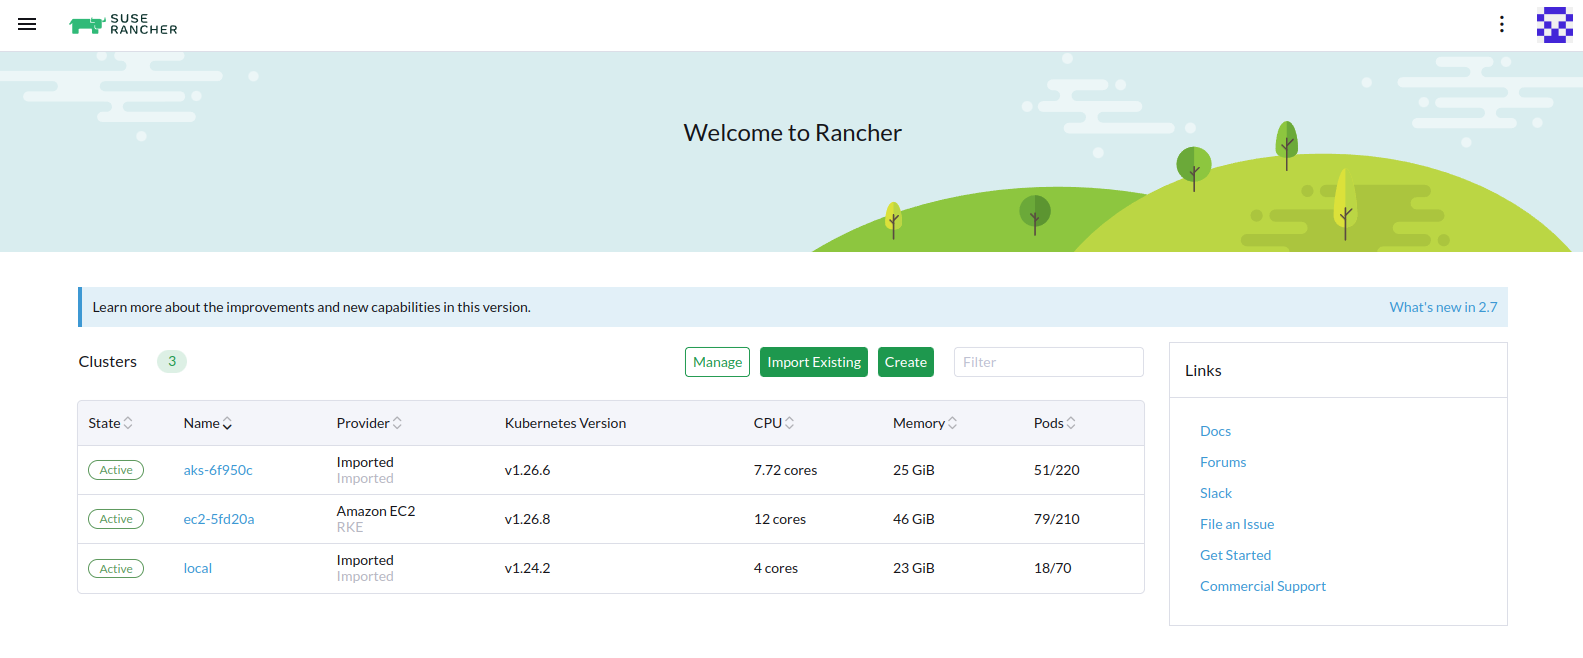
\includegraphics[width=\linewidth]{images/rancher-dashboard.png}
\label{fig:rancherDashboard}
\end{figure}

\subsubsection{CIS Benchmarks}

\subsubsection{CIS Benchmarks Installation}

\begin{lstlisting}[caption=Installing CIS, frame=single, basicstyle=\ttfamily]
# CIS Benchmarks
resource "rancher2_app_v2" "cisbench_fom" {
  lifecycle {
    ignore_changes = all
  }
  cluster_id = rancher2_cluster.cluster_fom.id
  name = "rancher-cis-benchmark"
  namespace = "cis-operator-system"
  project_id = data.rancher2_project.system.id
  repo_name = "rancher-charts"
  chart_name = "rancher-cis-benchmark"
  chart_version = var.cischart
}

\end{lstlisting}

\subsubsection{CIS Benchmark Reports}

\begin{itemize}
 \item AKS 1.0
 \item Kubernetes 1.6
\end{itemize}


%
%	Theorieteil
%

\pagebreak
\section{NIS2 Exploration}

\onehalfspacing

\subsection{NIS2 Article 21}

The NIS2 directive itself is a legal document organized into Chapters and Articles. It has a pan-European scope and targets critical businesses. Much of the content concerns reporting requirements and EU-wide cooperation and institutions, which we will not cover in this paper.\footnote{See \textit{EU (2022)}: NIS2 Directive. \cite{nis2}}

Article 21, however, defines the required Cybersecurity risk-management measures for critical infrastructure. In paragraph 2, point (g), NIS2 calls for basic cyber hygiene practices and cybersecurity training.

Any entity covered by the directive must, thus, have an IT Security Policy to implement basic cyber hygiene. To strengthen their security postures, entities could rely on one of the major frameworks and standards, such as the NIST SP 800 series, ISO/IEC 27001, Mitre Att\&ck, or CIS Controls.

The directive does not mandate whether an entity chooses one of these frameworks or creates its own policies. It also does not favor or champion any of the mentioned frameworks.

For this paper, we will focus on CIS Controls and the baselines provided by the CIS Benchmarks to fulfill Article 21's requirements.

\subsection{CIS Control 4}

The CIS Controls in the current version (v8) consist of 18 controls:

\begin{enumerate}
    \item Inventory and Control of Enterprise Assets
    \item Inventory and Control of Software Assets
    \item Data Protection
    \item Secure Configuration of Enterprise Assets and Software
    \item Account Management
    \item Access Control Management
    \item Continuous Vulnerability
    \item Audit Log Management
    \item Email and Web Browser Protections
    \item Malware Defenses
    \item Data
    \item Network Infrastructure
    \item Network Monitoring and Defense
    \item Security Awareness and Skills Training
    \item Service Provider
    \item Application Software Security
    \item Incident Response
    \item Penetration Testing\footnote{See \textit{CIS (2024)}: Critical Security Controls. \cite{cisControls}}
\end{enumerate}

As with the NIS2 articles, many of these controls are procedural and cannot be automated. Control 4, however, Secure Configuration of Enterprise Assets and Software, is of particular importance for individual IT systems, such as Kubernetes clusters.

Control 4 consists of several subcontrols:

\begin{enumerate}
    \item Establish and Maintain a Secure Configuration Process
    \item Establish and Maintain a Secure Configuration Process for
Network Infrastructure
    \item Configure Automatic Session Locking on Enterprise Assets
    \item Implement and Manage a Firewall on Servers
    \item Implement and Manage a Firewall on End-User Devices
    \item Securely Manage Enterprise Assets and Software
    \item Manage Default Accounts on Enterprise Assets and Software
    \item Uninstall or Disable Unnecessary Services on Enterprise Assets
and Software
    \item Configure Trusted DNS Servers on Enterprise Assets
    \item Enforce Automatic Device Lockout on Portable End-User Devices
    \item Enforce Remote Wipe Capability on Portable End-User Devices
    \item Separate Enterprise Workspaces on Mobile End-User Devices
\end{enumerate}

Control 4.1 strongly emphasizes the configuration process, as the default configuration for enterprise software is typically geared toward ease of deployment and use rather than security. This is where the CIS Benchmarks come into play.

\subsection{CIS Benchmarks for Kubernetes}

In general, key security risks with default configurations are:

\begin{itemize}
    \item Exposed Services and Ports
    \item Default Accounts and Passwords
    \item Pre-configured DNS Settings
    \item Older or Vulnerable Protocols
    \item Pre-installed Unnecessary Software
\end{itemize}

To mitigate these, the CIS Benchmarks provide a security baseline for enterprise software, such as Kubernetes, covering all aspects of CIS Control 4.1 and a matching IT Security Policy.\footnote{See \textit{CIS (2024)}: CIS Benchmarks List. \cite{cisBenchmarks}}

There are CIS Benchmarks tailored to the currently available and supported version of Kubernetes and the major hosted versions, such as the Azure Kubernetes Engine.

\subsection{CIS Kubernetes Benchmark Results}

Using the Rancher CIS Scans from above against a sample RKE2 Kubernetes cluster with default configuration, we receive the following results:



%
%	Praxisbezug
%

\pagebreak
\section{NIS2 Analysis}

\onehalfspacing

\subsection{Findings from the Kubernetes CIS Benchmark v1.8}

\subsection{Relevance for NIS2 Article 21}

\subsection{NIS2 Article 21 Compliance}

\subsection{Improving Compliance and mitigating the risks of attacks}



%
%	Fazit
%

\pagebreak
\section{Summary}

\onehalfspacing

Happy Ranching!


% Literaturverzeichnis
\cleardoublepage
\raggedright
\bibliographystyle{IEEEtranS}	% ieeetran verwenden, damit auch URLs angezeigt werden
\bibliography{seminar-lit}

\cleardoublepage
\justify
%
%	Ehrenwoertliche Erklaerung
%

\pagebreak

\pagenumbering{gobble} % Keine Seitenzahlen mehr
\onehalfspacing

%-----------------------------------
% Ehrenwoertliche Erklärung
%-----------------------------------
\section*{Declaration in lieu of oath}

\par\medskip

With this, I declare that I produced the submitted paper with no assistance from any other party and without the use of any unauthorized aids and, in particular, that I have marked as quotations all passages that are reproduced verbatim or near-verbatim from publications. Also, I declare that the submitted print version of this thesis is identical to its digital version. Further, I say that I have never introduced this thesis to any examination board in either its present form or in any other similar version. I herewith agree that you may publish this thesis. I herewith consent that you may upload this thesis to an external contractors' server to submit it to the contractors' plagiarism detection systems. Uploading this thesis to send it to plagiarism detection systems is not a form of publication.

\par\medskip
\par\medskip

\vspace{5cm}

\begin{table}[H]
	\begin{tabular*}{\textwidth}{c @{\extracolsep{\fill}} ccccc}
		Cologne, \the\month/\the\day/\the\year \\
		\rule[0.5ex]{12em}{0.55pt} & \rule[0.5ex]{12em}{0.55pt} \\
		(Location, Date) & (Signature)
	\end{tabular*}
\end{table}


\end{document}
